\chapter{Ferramentas de visualização de Redes Metabólicas}


\section{KEGG}

http:\/\/www.kegg.jp\/ -> \\ Data-oriented entry points  -> \\KEGG PATHWAY ->\\ Pathway Maps -> \\1. Metabolism  -> \\1.0 Global and overview maps / Metabolic pathways

\begin{figure}[h]
\centering
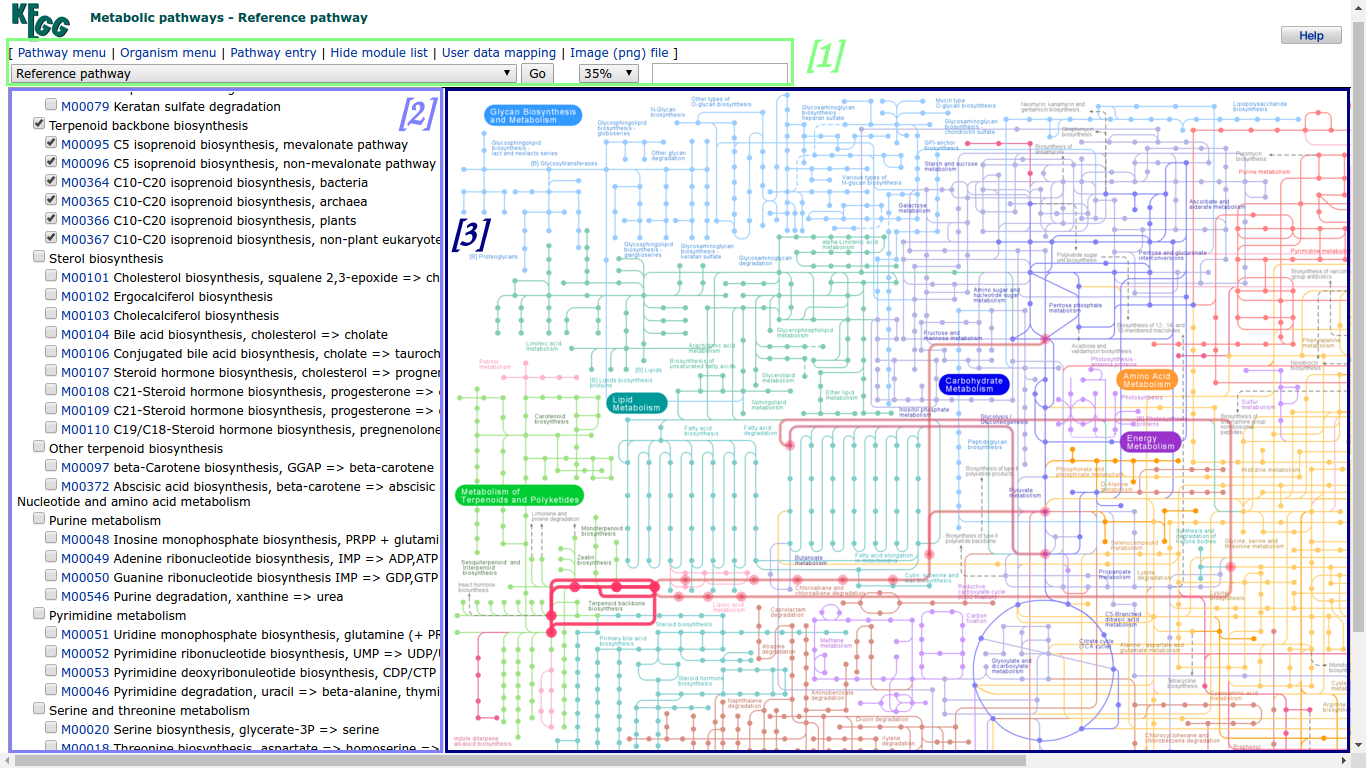
\includegraphics[width=1\textwidth]{terpenoidBackboneKEGG_id.png}
\caption{Visão geral da rede metabólica de referência do KEGG, com destaque na via metabólica de biossíntese do \textit{backbone} de terpenóides. (1), (2) e (3).}
\label{terpenoidBackboneKEGG}
\end{figure}


Notação: http:\/\/www.genome.jp\/kegg\/document\/help\_pathway.html



http:\/\/www.kegg.jp\/ -> \\ Data-oriented entry points  -> \\KEGG PATHWAY ->\\ Pathway Maps -> \\1. Metabolism/Terpenoid/PK   -> \\1.9 Metabolism of terpenoids and polyketides / Terpenoid backbone biosynthesis

\begin{figure}[h]
\centering
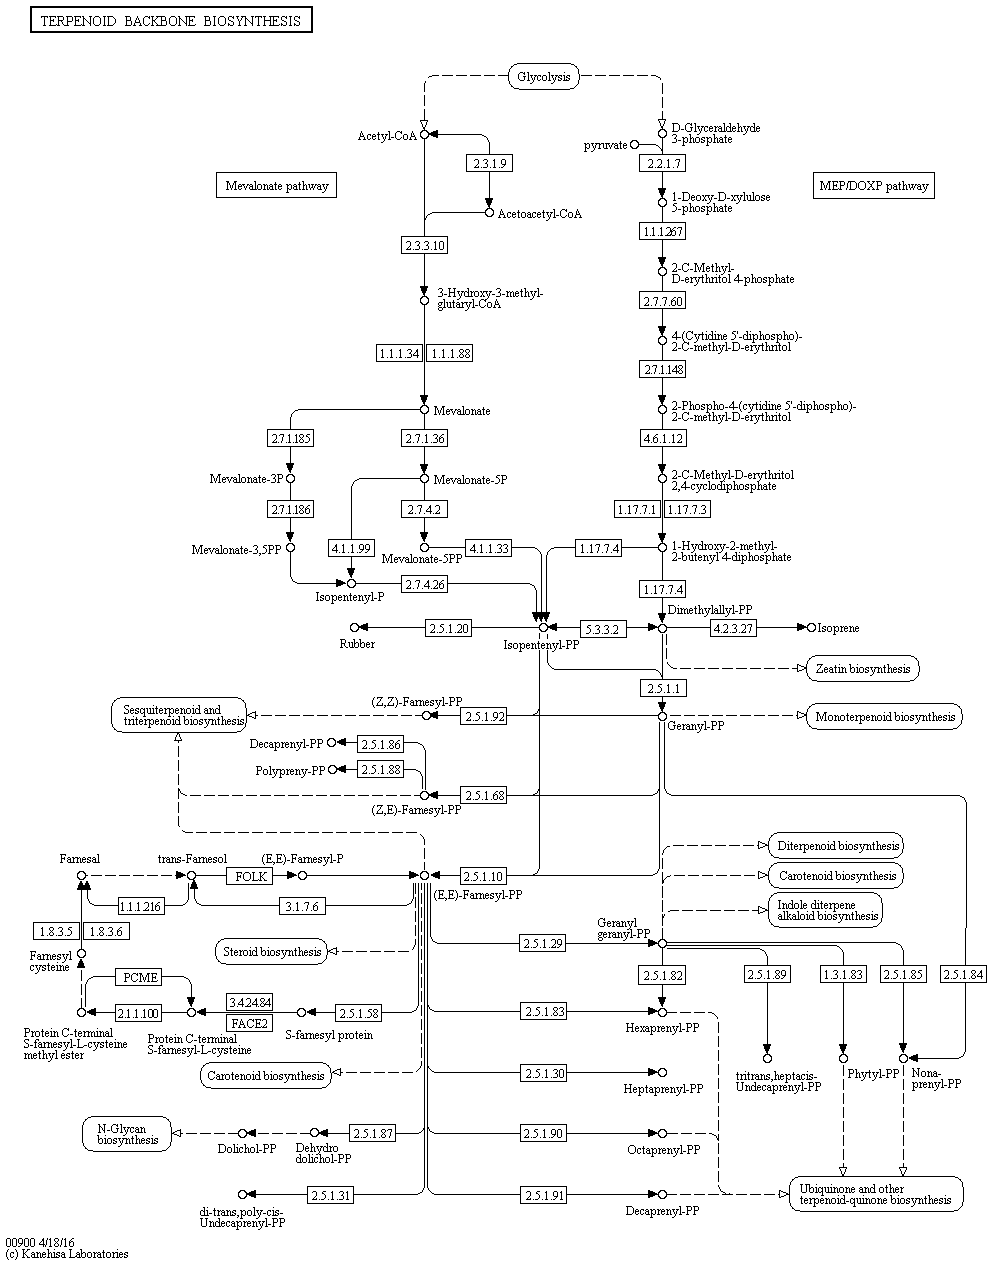
\includegraphics[width=1\textwidth]{terpenoidViaKEGG.png}
\caption{Via metabólica de biosíntese do \textit{backbone} de terpenóides}
\label{terpenoidBackboneKEGG}
\end{figure}


Tipo de arquivo:
Objetos clicáveis, setas e containers com significado (Notação: http:\/\/www.genome.jp\/kegg\/document\/help\_pathway.html), minimapa ao passar mouse por cima de vias representadas por nós, etc

\section{MetaCyc}


Figura do capitulo anterior: bioluminescencia.

\begin{figure}[h]
\centering
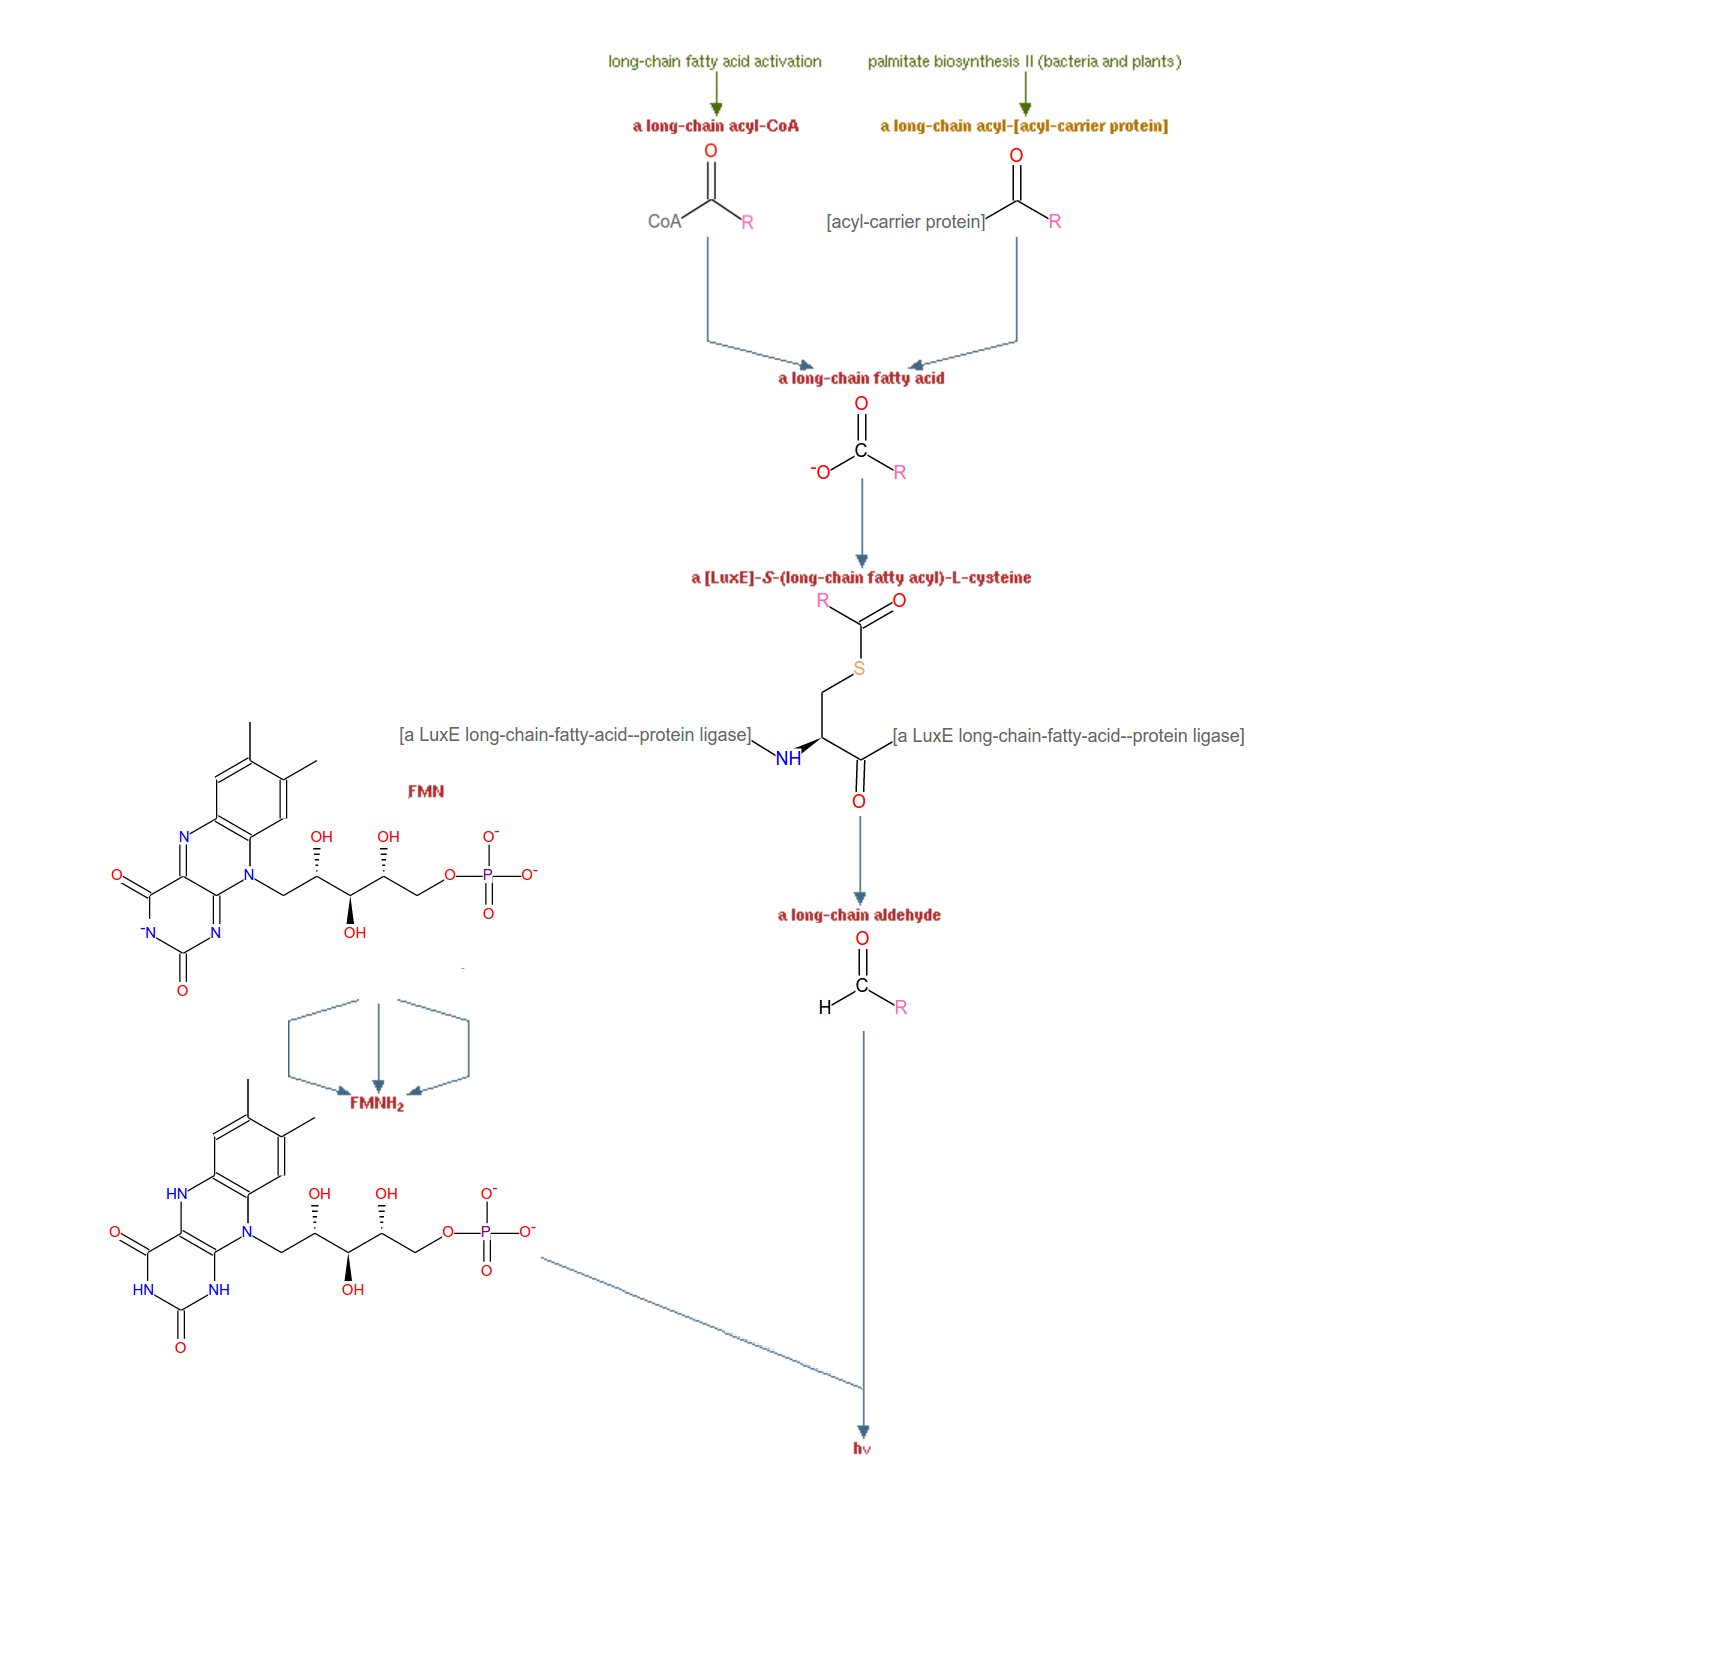
\includegraphics[width=1.2\textwidth]{bioLuz_modificado.png}
\caption{Mesa figura do capitulo 1, mas com maior nível de detalhes}
\label{terpenoidBackboneKEGG}
\end{figure}

\section{Reactome Browser}

\section{Cytoscape}

%\cite{lacroixCTS08}